

%This document provides an introduction to statistical disclosure control (SDC)
%and guidelines on how to apply SDC methods to microdata. Section 1 introduces
%basic concepts and presents a general workflow. Section 2 discusses methods of
%measuring disclosure risks for a given micro dataset and disclosure scenario. Sec-
%tion 3 presents some common anonymization methods. Section -1 introduces how
%to assess utility of a micro dataset after applying disclosure limitation methods.
\documentclass{beamer}

\usepackage{amsmath}
\usepackage{amssymb}
\usepackage{subfiles}
\usepackage{graphicx}

\begin{document}
\begin{frame}
	\frametitle{Statistical Disclosure Control}
	\begin{itemize}
		\item Official Statistics and Survey Methodology
		\item Numerous Topics including:
		\item Martin Templ (Univ. of Vienna)
		\item The \textbf{sdcMicro} package
		\item (R Conference in Romania)
	\end{itemize}
\end{frame}

%====================================================== %
\begin{frame}
	\frametitle{Official Statistics}
	\begin{quotation}
		\noindent Official statistics are statistics published by government agencies or other public bodies such as international organizations. They provide quantitative or qualitative information on all major areas of \textbf{citizens' lives}, such as economic and social development, living conditions,health, education, and the environment.\\ (Wikipedia)
	\end{quotation}
	
	\begin{itemize}
		\item Remark: Are we talking about data about individual people?
	\end{itemize}
\end{frame}
%====================================================== %
\begin{frame}
	\frametitle{Official Statistics}
	\begin{quotation}
		"Personally identifiable information" (PII), as used in US privacy law and information security, is information that can be used on its own or with other information to identify, contact, or locate a single person, or to identify an individual in context. 
	\end{quotation}
\end{frame}
%====================================================== %
\begin{frame}
	\frametitle{Official Statistics}
	\begin{quotation}
		\noindent  PII is "any information about an individual maintained by an agency, including \\ (1) any information that can be used to distinguish or trace an individual‘s identity, such as name, social security number, date and place of birth, mother‘s maiden name, or biometric records; and \\ (2) any other information that is linked or linkable to an individual, such as medical, educational, financial, and employment information."
	\end{quotation}
	(NIST Special Publication 800-122)
\end{frame}

\begin{frame}
	\begin{itemize}
		\item 
		\item \textbf{De-anonymization} is the reverse process in which anonymous data is cross-referenced with other data sources to re-identify the anonymous data source.
	\end{itemize}
\end{frame}
%====================================================== %
\begin{frame}
	Celebrities since 1950 (may be deceased )
	\begin{itemize}
		\item US, Born in 1935,  identical twin, other twin deceased.
		% \item US, Bell's Palsy
		\item US, Redhaired, 6"4'
		\item UK, Greek Cypriot Heritage, Convert to Islam
		\item UK, Female, amputation of left leg below the knee
		\item Irish, Male, Blond-haired, Mullingar
		\item USA, Married to UK based Lawyer.
		\item UK, Same Sex Marriage, 27 years older than husband.
		\item Mexican, Irish Heritage
	\end{itemize}
	
\end{frame}


%====================================================== %
\begin{frame}
	\begin{figure}
		\centering
		
\includegraphics[width=1.1\linewidth]{./JPEGS/Slide1}
	\end{figure}
\end{frame}
%====================================================== %
\begin{frame}
	\begin{figure}
		\centering
		
\includegraphics[width=1.1\linewidth]{./JPEGS/Slide2}
	\end{figure}
\end{frame}
\begin{frame}
	\begin{figure}
		\centering
		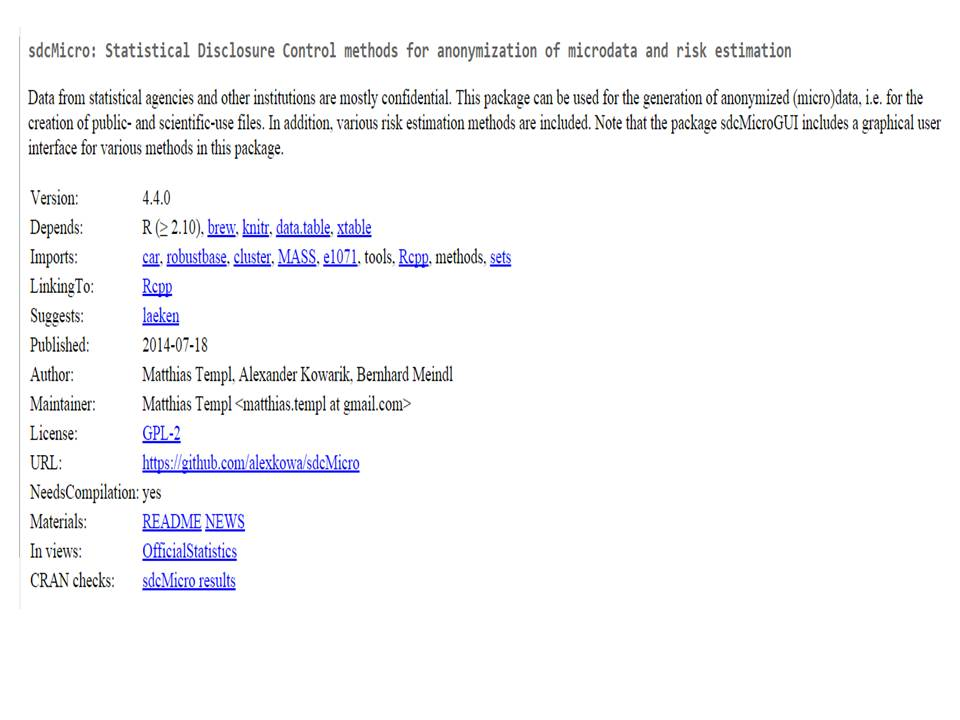
\includegraphics[width=1.1\linewidth]{./JPEGS/Slide3}
		
	\end{figure}
\end{frame}
%====================================================== %
\begin{frame}
	\begin{figure}
		\centering
		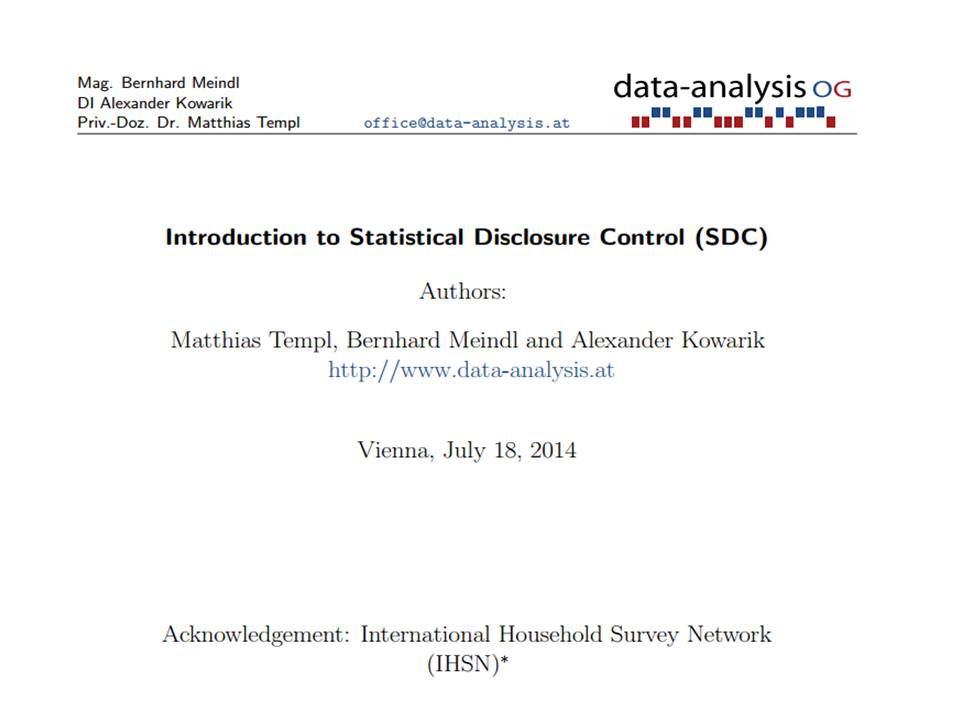
\includegraphics[width=1.1\linewidth]{./JPEGS/Slide4}
	\end{figure}
\end{frame}
\begin{frame}

\frametitle{Microdata}
\textbf{MicroData}
\begin{itemize}
	\item
A microdata file is a dataset that holds information collected on individual units;
examples of units include people, households or enterprises. 
\item For each unit, a set of
variables is recorded and available in the dataset. 
%\item This section discusses concepts
%related to disclosure and SDC methods, and provides a workfiow that shows how
%to apply SDC methods to microdata.
\end{itemize}
\end{frame}
\begin{frame}
	\frametitle{Statistical Disclosure Control - Concepts}
	\Large
	\begin{itemize}
		\item[(1)] 	
		A \textbf{microdata file} is a dataset that holds information collected on individual units;
		examples of units include people, households or enterprises.\\ For each unit, a set of
		variables is recorded and available in the dataset.
		\item[(2)] A \textbf{disclosure risk} occurs if an unacceptably narrow estimation of a respondent’s confidential information is possible or if exact disclosure is possible with a high level of confidence.
	\end{itemize}
\end{frame}

\section*{Disclosure Types}
%====================== %
\begin{frame}
	\textbf{Identity disclosure:}
	\begin{itemize}
		\item In this case, the intruder associates an individual with a released data record that contains sensitive information, i.e. linkage with ex-
		ternal available data is possible.
		\item Identity disclosure is possible through direct
		identifiers, rare combinations of values in the key variables and exact knowl-
		edge of continuous key variable values in external databases. 
		\item For the latter,
		extreme data values (e.g., extremely high turnover values for an enterprise)
		lead to high re-identification risks, i.e. it is likely that responends with ex-
		treme data values are disclosed.
	\end{itemize}
\end{frame}
% Page 2 / 31
% 1 CONCEPTS
%====================== %
\begin{frame}
	\textbf{Attribute disclosure:}
	\begin{itemize}
		\item In this case, the intruder is able to determine some charac-
		teristics of an individual based on information available in the released data.
		\item For example, if all people aged 56 to GO who identify their race as black in
		region 12345 are unemployed, the intruder can determine the value of the
		variable labor status.
	\end{itemize}
\end{frame}
%====================== %
\begin{frame}
	\textbf{Inferential disclosure:}
	\begin{itemize}
		
		\item In this case, the intruder, though with some uncertainty,
		can predict the value of some characteristics of an individual more accu-
		rately with the released data.
	\end{itemize}
\end{frame}
%=====================================%	
\begin{frame}
	\frametitle{Statistical Disclosure Control - Concepts}
	
	\begin{itemize}
		\item Removing and encrypting are only acceptable ways for disclosure control of identifier values. 
		\item For 
		another types of attributes we can apply masking methods.
		\item  They can in turn be divided on two groups 
		depending on their effect on the original data . 
	\end{itemize}
	
\end{frame}
%=====================================%

\begin{frame}
	
	\begin{description}
		\item[Perturbative methods.] The original microfile is distorted, but in such a way that a difference between 
		values of statistical rates of masking and original data would be acceptable. 
		\item[Non-perturbative methods.] They protect data without altering them. Non-perturbative methods base on 
		principles of suppression and generalization (recoding). 
	\end{description}
\end{frame}
%=====================================%

\begin{frame}
	
	\begin{itemize}
		\item Suppression is a removing some data from original 
		set. 
		\item Recoding is a data enlargement. 
		\item In case of continuous data (for example, age) non-perturbative methods 
		can transform it to interval, fuzzy or categorical datatype.
	\end{itemize}
	
	
	
\end{frame}
\begin{frame}
	%-------------------------------------%
	Sometimes methods generating synthetic data or combined methods are also applied. Such methods 
	are not acceptable at microdata preparation, because if we don’t know the aim of the follow-up analysis, we 
	can not generate adequate set of \textbf{synthetic data}. 
\end{frame}
%================================================================== %
\subsection*{1.1. Categorization of Variables}
\begin{frame}
\frametitle{Types of variables}

In accordance with disclosure risks, variables can be classified into three groups,
which are not necessarily exclusive:

\bigskip
\begin{description}
	\item[Direct Identifiers] are variables that precisely identify statistical units. 
\end{description}

\begin{itemize}
	\item For example, social insurance numbers, names of companies or persons and addresses
	are direct identifiers 
	\item (Remark: Primary Keys)
\end{itemize}
\end{frame}
%======================================================================== %
\begin{frame}
\frametitle{Types of variables}
\begin{description}
	\item[Key variables] are a set of variables that, when considered together, can be used
	to identify individual units. For example, it may be possible to identify
	individuals by using a combination of variables such as gender, age, region
	and occupation. Other examples of key variables are income, health status,
	nationality or political preferences. 
\end{description}
\end{frame}
%======================================================================== %
\begin{frame}
	\frametitle{Types of variables}
\begin{itemize}
	\item Key variables are also called implicit
	identifiers or quasi-identifiers. \item When discussing SDC methods, it is preferable
	to distinguish between categorical and continuous key variables based on the
	scale of the corresponding variables.
	\item Non-identifying variables are variables that are not direct identifiers or key variables.
\end{itemize}
%======================================================= %
%For specific methods such as l-diversity, another group of sensitive variables is defined in Section 
\end{frame}
\subsection*{1.2. What is disclosure?}
\begin{frame}
\frametitle{Types of Disclosure}

\begin{itemize}
\item In general, disclosure occurs when an intruder uses the released data to reveal
previously unknown information about a respondent.
\item There are three different types of disclosure:\textit{(next set of slides)}
\end{itemize}


\end{frame}
%==================================================================== %
\begin{frame}
	\frametitle{Types of Disclosure}

\textbf{Identity disclosure:}
\begin{itemize}
	\item In this case, the intruder associates an individual with a re-
	leased data record that contains sensitive information, i.e. linkage with external available data is possible.
	\item Identity disclosure is possible through direct
	identfiers, rare combinations of values in the key variables and exact knowledge of continuous key variable values in external databases. 
	\item For the latter,
	extreme data values 
	lead to high re-identification risks, i.e. it is likely that responends with extreme data values are disclosed.
\end{itemize}
% - (e.g., extremely high turnover values for an enterprise)
\end{frame}
%==================================================================== %
\begin{frame}
	\frametitle{Types of Disclosure}
\textbf{Attribute disclosure:}
\begin{itemize}
	
	\item In this case, the intruder is able to determine some characteristics of an individual based on information available in the released data.
	\item For example, if all people aged 56 to GO who identify their race as black in
	region 12345 are unemployed, the intruder can determine the value of the
	variable labor status.
	\item \textbf{Also} Diet - detailed questionnaire on diet can give clues to other aspects of some people's lives.
\end{itemize}
\end{frame}
%==================================================================== %
\begin{frame}
	\frametitle{Types of Disclosure}
\textbf{Inferential disclosure:}
\begin{itemize}
	
	\item In this case, the intruder, though with some uncertainty,
	can predict the value of some characteristics of an individual more accurately with the released data.
\end{itemize}
\end{frame}
%==================================================================== %
\begin{frame}
\frametitle{Linkage}
\textbf{Linkage}
\begin{itemize}
	
\item If linkage is successful based on a number of identifiers, the intruder will have
	access to all of the information related to a specific corresponding unit in the
	released data. 
\item This means that a subset of critical variables can be exploited to
	disclose everything about a unit in the dataset.
\end{itemize}

\end{frame}
	\begin{frame}
		\frametitle{sdcMicro}
		\begin{itemize}
			\item The \texttt{R} package \textbf{sdcMicro} is a well-known collection of microdata protection methods developed by \textbf{Statistics Austria}, which is already in use in several national statistics offices. 
			\item \textbf{sdcMicro} has become one of the standard tools for \textbf{microdata protection} during the last five years.
			\item The IHSN is supporting the further development of sdcMicro and has partnered with its developers to perform the following tasks (next slide).
		\end{itemize}
	\end{frame}
	\begin{frame}
		\begin{itemize}
			\item Version 4.4.0 of the sdcMicro package is available on the Comprehensive R Archive Network (CRAN).
			\item Existing guidelines and a user guide for \textbf{sdcMicro} are being updated. 
			\item A specific tutorial is being developed to show how to implement these concepts and algorithms on real datasets (see 
			Vignettes)
		\end{itemize}
		
		
	\end{frame}
	%======================================================= % 
	\begin{frame}
		\frametitle{\texttt{R}-Package sdcMicro and sdcMicroGUI}
		
		\begin{itemize}
			\item SDC methods introduced in this guideline can be implemented by the R-Package
			sdcMicro. 
			\item Users who are not familiar with the native R command line interface
			can use sdcMicroGUI, an easy-to-use and interactive application. 
			%For details, see Tcnipl ct al. [2Ol'lb, 2013].
		\end{itemize}
	\end{frame}
	%=========================================================== %
	%\section*{1.3. Remarks on SDC Methods}
	\begin{frame}
		\frametitle{SDC Methods} 
		\textbf{Mathematical Foundation of SDC}
		\begin{itemize}
			\item In general, SDC methods borrow techniques from other fields. 
			\item For instance, multivariate (robust) statistics are used to modify or simulate continuous variables and
			to quantify information loss. 
			
			\item Distribution-fitting methods are used to quantify
			disclosure risks.
			\item Statistical modeling methods form the basis of perturbation algorithms, to simulate synthetic data, to quantify risk and information loss. 
			\item Linear
			programming is used to modify data but minimize the impact on data quality.
		\end{itemize}
	\end{frame}
	%==================================================================== %
	\begin{frame}
		\frametitle{SDC Methods} 
		\begin{itemize}
			\item
			Problems and challenges arise from large datasets and the need for efficient algorithms and implementations.\\ (\textbf{Remark} 1000 variables+)
			\item Another layer of complexity is produced by complex
			structures of hierarchical, multidimensional data sampled with complex survey designs. \\ (\textbf{Remark} Rooted Questions )
			\item 
			Missing values are a challenge, especially for computation time issues; structural Zeros (values that are by definition Zero) also have impact on the application
			of SDC methods. 
		\end{itemize}
	\end{frame}
	%================================================================================ %
	\begin{frame}
		\frametitle{SDC Methods} 
		Furthermore, the compositional nature of many components
		should always be considered, but adds even more complexity.\\ \bigskip
		SDC techniques can be divided into three broad topics:
		\begin{itemize}
			\item Measuring disclosure risk % (see Section 2)
			\item Methods to anonymize micro-data % (see Section 3)
			\item Comparing original and modified data (information loss) % (see Section /l)
		\end{itemize}
	\end{frame}
	%============================================================================== %
%============================================== %
\begin{frame}
	\frametitle{Risk Versus Data Utility}
	The goal of SDC is always to release a safe micro dataset with high data utility and
	a low risk of linking confidential information to individual respondents. Figure 1
	shows the trade-off between disclosure risk and data utility. 
	% We applied two SDC methods with different parameters to the European Union Structure of Earnings
	% Statistics (SES) data [see Tenipl ct al., 2014-<1, for more on anonymization of this
	% dataset].
	
\end{frame}

%============================================== %
\begin{frame}
	\begin{figure}
		\centering
		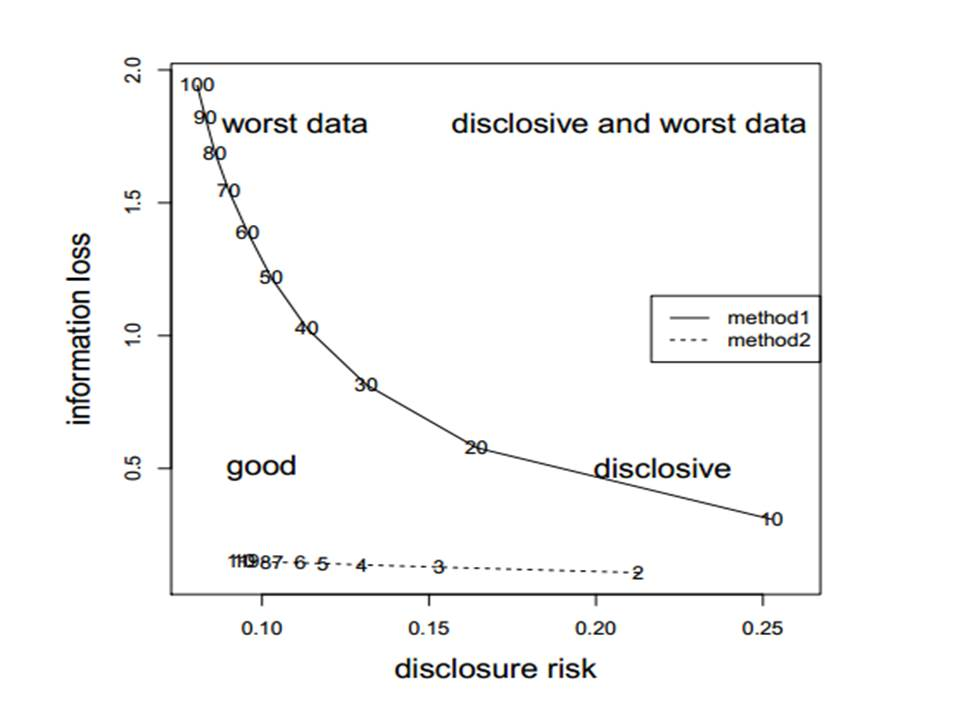
\includegraphics[width=0.99\linewidth]{JPEGS/TemplGraph1}
	\end{figure}
	
\end{frame}
%============================================== %
\begin{frame}
	\frametitle{Risk Versus Data Utility}
	\begin{itemize}
		\item For Method 1 (in this example adding noise), the parameter varies between 10
		(small perturbation) to 100 (perturbation is 10 times higher). 
		\item When the parameter
		value is 100, the disclosure risk is low since the data are heavily perturbed, but the
		
		information loss is very high, which also corresponds to very low data utility. 
	\end{itemize}
	
	%--------------------------Page 3 / 31
	%% 1 CONCEPTS
\end{frame}
%============================================== %
\begin{frame}
	\frametitle{Risk Versus Data Utility}
	\begin{itemize}
		\item When
		only low perturbation is applied to a dataset, both risk and data utility are high. 
		\item It
		is easy to see that data anonymized with Method 2 (we used microaggregation with
		different aggregation levels) have considerably lower risk; therefore, this method
		is preferable.
	\end{itemize}
\end{frame}
%============================================== %
\begin{frame}
	\frametitle{Risk Versus Data Utility}
	\begin{itemize}
		\item In addition, information loss increases only slightly if the parameter
		value increases; therefore, Method 2 with parameter value of approximately 7
		would be a good choice in this case since this provides both, low disclosure risk
		and low information loss. 
	\end{itemize}
\end{frame}
%============================================== %
\begin{frame}
	\frametitle{Risk Versus Data Utility}
	\begin{itemize}
		\item For higher values, the perturbation is higher but the
		gain is only minimal, lower values reports higher disclosure risk, Method 1 should
		not be chosen since the disclosure risk and the information loss is higher than for
		method 2. \item However, if for some reasons method 1 is chosen, the parameter for
		perturbation might be chosen around 40 if 0.1 risk is already considered to be
		safe. 
		\item For data sets concerning very sensible information (like cancer) the might
		be, however, to high risk and a perturbation value of 100 or above should then be
		chosen for method 1 and a parameter value above 10 might be chosen for method
	\end{itemize}
\end{frame}
%============================================== %
%\begin{frame}
%\begin{itemize}
%\item Figure 1: Risk versus information loss obtained for two specific perturbation meth-
%ods and different parameter choices applied to SES data o11 continuous
%scaled variables. Note that the information loss for the original data is
%O and the disclosure risk is 1 respecively, i.e. the two curves starts from
%(1,0).
%\end{itemize}
%\end{frame}
%============================================== %
\begin{frame}
	\textbf{Considerations}
	\begin{itemize}
		\item In real-world examples, things are often not as clear, so data anonymization specialists should base their decisions regarding risk and data utility on the following
		considerations:
		%Page 4 / 31
		%
		%
		%
		%1 CONCEPTS
		
		\item What is the legal situation regarding data privacy? Laws on data privacy vary
		between countries; some have quite restrictive laws, some don’t, and laws often
		differ for different kinds of data (e.g., business statistics, labor force statistics,
		social statistics, and medical data).
		
	\end{itemize}
\end{frame}
%============================================== %
\begin{frame}
	\begin{itemize}
		
		\item How sensitive is the data information and who has access to the anonymized
		data file? Usually, laws consider two kinds of data users: users from universities
		and other research organizations, and general users, i.e., the public. In the first
		case, special contracts are often made between data users and data producers.
		
		\item Usually these contracts restrict the usage of the data to very specific purposes, and
		allow data saving only within safe work environments. For these users, anonymized
		microdata files are called scientific use files, whereas data for the public are called
		public use files. Of course, the disclosure risk of a public use ile needs to be very
		low, much lower than the corresponding risks in scientific use files. For scientific
		use files, data utility is typically considerably higher than data utility of public use
		files.
		
	\end{itemize}
\end{frame}
%============================================== %
\begin{frame}
	\begin{itemize}
		\item Another aspect that must be considered is the sensitivity of the dataset. Data
		011 individuals’ medical treatments are more sensitive than an establishment’s
		turnover values and number of employees. If the data contains very sensitive in-
		formation, the microdata should have greater security than data that only contain
		information that is not likely to be attacked by intruders.
	\end{itemize}
\end{frame}
%============================================== %
\begin{frame}
	\begin{itemize}
		\item Which method is suitable for which purpose? Methods for Statistical Disclosure Control always imply to remove or to modify selected variables.
		\item \textbf{Key} The data
		utility is reduced in exchange of more protection. 
		\item While the application of some
		specific methods results in low disclosure risk and large information loss, other
		methods may provide data with acceptable, low disclosure risks. 
		
	\end{itemize}
\end{frame}
%============================================== %
\begin{frame}
	\textbf{Recommendations (or lack thereof)}
	\begin{itemize}
		\item General recomendations can not be given here since the strenghtness and weakness of methods
		depends on the underlying data set used.
		\item  Decisions on which variables will be
		modified and which method is to be used result are partly arbitrary and partly
		result from a prior knowledge of what the users will do with the data.
	\end{itemize}
\end{frame}
%============================================== %
\begin{frame}
	\begin{itemize}
		\item Generally, when having only few categorical key variables in the data set, recoding and local suppression to achieve low disclosure risk for categorical key
		variables is recommended. 
		\item In addition, in case of continous scaled key variables,
		microaggregation is easy to apply and to understand and gives good results.
		\item  For
		more experienced users, shuffling may often give the best results as long a strong
		relationship between the key variables to other variables in the data set is present.
		
	\end{itemize}
\end{frame}
%============================================== %
\begin{frame}
	\begin{itemize}
		\item In case of many categorical key variables, post—randomization might be applied
		to several of these variables. Still methods, such as post—randomization (PRAM),
		may provide high or low disclosure risks and data utility, depending on the specific
		choice of parameter values, e.g. the swapping rate.
	\end{itemize}
\end{frame}
%============================================== %
\begin{frame}
	\begin{itemize}
		\item Beside these recommendations, in any case, data holders should always estimate
		the disclosure risk for their original datasets as well as the disclosure risks and
		data utility for anonyrnized versions of the data. 
		\item To achieve good results (i.e., low
		disclosure risk, high data utility), it is necessary to anonyrnize in an explanatory
		manner by applying different methods using different parameter settings until a
		suitable trade-off between risk and data utility has been achieved.
	\end{itemize}
\end{frame}
\end{document}